\section{Evaluation}
\label{sec:eval}

\subsection{Experimental Setup}
Table~\ref{tab:setup} summarizes the machine used in our experiments.

% 表格請用 booktabs；表格內文字不可小於 8pt（勿用 \tiny、\scriptsize）
\begin{table}[t]
  \caption{Experimental platform.}
  \label{tab:setup}
  \begin{tabular}{ll}
    \toprule
    Component & Specification \\
    \midrule
    CPU       & 2$\times$ 16-core x86-64 @ 2.5\,GHz \\
    Memory    & 256\,GB DDR5 \\
    Compiler  & GCC 13.2, \texttt{-O3} \\
    \bottomrule
  \end{tabular}
\end{table}

\subsection{Scalability}
Figure~\ref{fig:speedup} shows the speedup of \sys over the baseline.

% 單欄圖用 figure；跨雙欄用 figure*
% 圖中文字需 >= 8pt：產生圖時請以實際刊出寬度（單欄約 3.33 in）設定字級，
% 不要把大圖用 \includegraphics 縮小。
\begin{figure}[t]
  \centering
  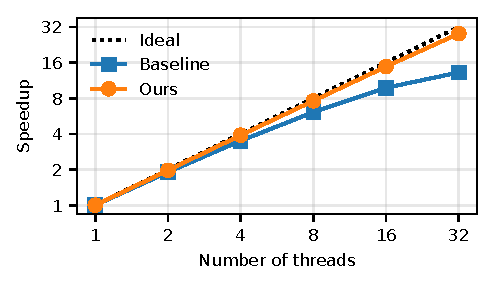
\includegraphics[width=\columnwidth]{speedup}
  \caption{Speedup on 1--32 threads (higher is better).}
  % \Description 是 ACM 要求的無障礙替代文字，不會印在 PDF 上
  \Description{Line chart of speedup versus thread count; Ours scales
    close to ideal while the baseline flattens after 8 threads.}
  \label{fig:speedup}
\end{figure}
